I investigate the causal effect of rainfall on labor supply decisions in the Sao Paulo Metropolitan Region (RMSP), Brazil. Specifically, I examine whether precipitation affects both the probability of working and commute time for work-related activities. Weather conditions may influence work decisions through multiple channels: transportation costs and delays, direct utility effects from weather preferences, and productivity considerations. Understanding these relationships has important implications for labor market policy and urban planning, particularly in large metropolitan areas where weather-related disruptions can have significant economic consequences. My analysis contributes to the growing literature on environmental factors and labor market outcomes by providing evidence from one of the largest urban agglomerations in the developing world.

My research relates to several strands of economic literature. First, it builds on the extensive literature examining labor supply responses to various shocks and constraints, including transportation costs \citep{zenou2009urban}, weather conditions \citep{connolly2008here}, and urban characteristics \citep{moretti2011local}. Second, my work contributes to the emerging field of environmental economics that studies how weather and climate affect economic outcomes \citep{hsiang2016climate}. Previous studies have found mixed evidence on weather effects on labor supply: some find negative effects of extreme weather on work attendance \citep{lee2016temperature}, while others document positive effects through reduced leisure alternatives \citep{connolly2008here}. Third, I add to the literature on developing country labor markets, where informal employment and flexible work arrangements may lead to different responses to weather shocks compared to developed economies. My focus on Brazil is particularly relevant given its large informal sector and the importance of weather-sensitive outdoor work.

My rainfall data comes from the Centro Nacional de Monitoramento e Alertas de Desastres Naturais (CEMADEN), Brazil's national center for monitoring and alerting natural disasters. CEMADEN operates a comprehensive network of automatic weather stations throughout Brazil, providing high-frequency precipitation measurements. For the RMSP, I utilize daily rainfall data from 2017, which covers the period of my labor market survey. The CEMADEN data offers several advantages: it provides precise temporal coverage matching my survey period, has wide spatial coverage across the metropolitan region, and uses standardized measurement protocols ensuring data quality. I aggregate daily rainfall measurements to match the survey reference periods, creating variables for total rainfall (in millimeters) and a binary indicator for any precipitation. This approach allows me to capture both the extensive margin (occurrence of rainfall) and intensive margin (amount of rainfall) effects on labor supply decisions. Figure \ref{fig:hist} shows the distribution of rainfall in my sample.

My primary labor market data comes from the 2017 Origin-Destination Survey (Pesquisa Origem-Destino) conducted by the Sao Paulo Metropolitan Transportation Company (Companhia do Metropolitano de Sao Paulo). This comprehensive household survey collects detailed information on travel patterns, work activities, and demographic characteristics for residents of the RMSP. For each individual, I observe the complete set of trips made during a reference day, including the origin and destination zones for each segment of their trajectory and the stated purpose for each trip. This allows me to reconstruct the full sequence of movements throughout the day and to identify work-related travel with spatial precision. The survey covers approximately 32,000 individuals and provides rich information on individual work decisions, commute times in minutes, and socioeconomic characteristics. Figure \ref{fig:hist} also displays the distributions of number of trips and commute durations in my dataset.

To combine the rainfall and labor market data, I developed a spatial matching procedure that links survey respondents to weather station measurements. I first calculated the geographic centroids of each origin-destination zone in the survey using municipal boundaries and zone definitions. Next, I created Voronoi polygons around each CEMADEN weather station, which partition the metropolitan area such that each location is assigned to its nearest weather station. I then matched each survey respondent's zone centroid to the corresponding weather station, assigning them the rainfall measurements from their nearest station. This approach ensures that each individual receives rainfall data from the most geographically relevant weather station while maintaining the spatial precision necessary for causal identification. The matching process accounts for the irregular spatial distribution of weather stations and survey zones. Figure \ref{fig:rmsp_voronoi} illustrates my spatial matching strategy, showing both the RMSP zone partitions and the Voronoi diagram I constructed.

I employ a reduced-form approach that exploits plausibly exogenous variation in daily rainfall to identify causal effects on labor supply. I estimate the following models for work probability and commute time:
\begin{align*}
Y_{iz} &= \alpha + \beta_1 \text{Rain}_{iz} + \beta_2 \text{Rainfall}_{iz} + \mathbf{X}_{iz}'\gamma + \delta_z + u_{iz}
\end{align*}
where $Y_{iz}$ represents either a binary work indicator or commute time for individual $i$ in zone $z$, $\text{Rain}_{iz}$ is a dummy for any precipitation, $\text{Rainfall}_{iz}$ is total rainfall in millimeters, $\mathbf{X}_{iz}$ includes individual controls, and $\delta_z$ represents zone fixed effects. I estimate five specifications with progressively more controls: rainfall dummy only, rainfall amount only, both rainfall variables, both plus individual controls, and the full specification with zone fixed effects. The identifying assumption is that daily rainfall variation is exogenous to individual labor supply decisions, which is plausible given the short-term nature of weather variation and the difficulty of perfectly predicting daily precipitation.

My empirical analysis reveals null effects of rainfall on both the extensive and intensive margins of labor supply in the RMSP. For work probability, the estimated effect of rainfall is zero across all model specifications, indicating no impact of precipitation on the likelihood of working. For commute time, rainfall does not increase travel duration; in fact, the point estimate is negative and statistically significant in some specifications, suggesting a small reduction in commute time on rainy days. However, these effects are not robust across all models and are not economically meaningful. Overall, I find no evidence that rainfall affects either the probability of working or the duration of work-related commutes, as shown in Tables \ref{tab:panel_a} and \ref{tab:panel_b}.

These results indicate that daily rainfall variation does not substantially influence short-term labor supply decisions in this urban Brazilian context. The findings hold across different model specifications, including those with comprehensive individual controls and zone fixed effects, and suggest that neither the extensive effect (raining or not) nor the intensive effect (amount of rainfall) significantly alters work behavior or commute times.  

There are several limitations to this analysis. First, the correlation of rainfall across different zones in Sao Paulo is high, so the identification relies primarily on between-day variation rather than within-day or within-city variation. As the data covers only weekdays for a single year, this may limit the amount of variation in outcomes. Second, the analysis does not capture the effects of extreme weather events such as flooding, which may have more pronounced impacts on labor market outcomes and urban infrastructure. Future research could investigate the effects of such disasters, as well as explore heterogeneous impacts across formal and informal labor markets, or between central and peripheral urban areas.

\begin{figure}[H]
    \centering
    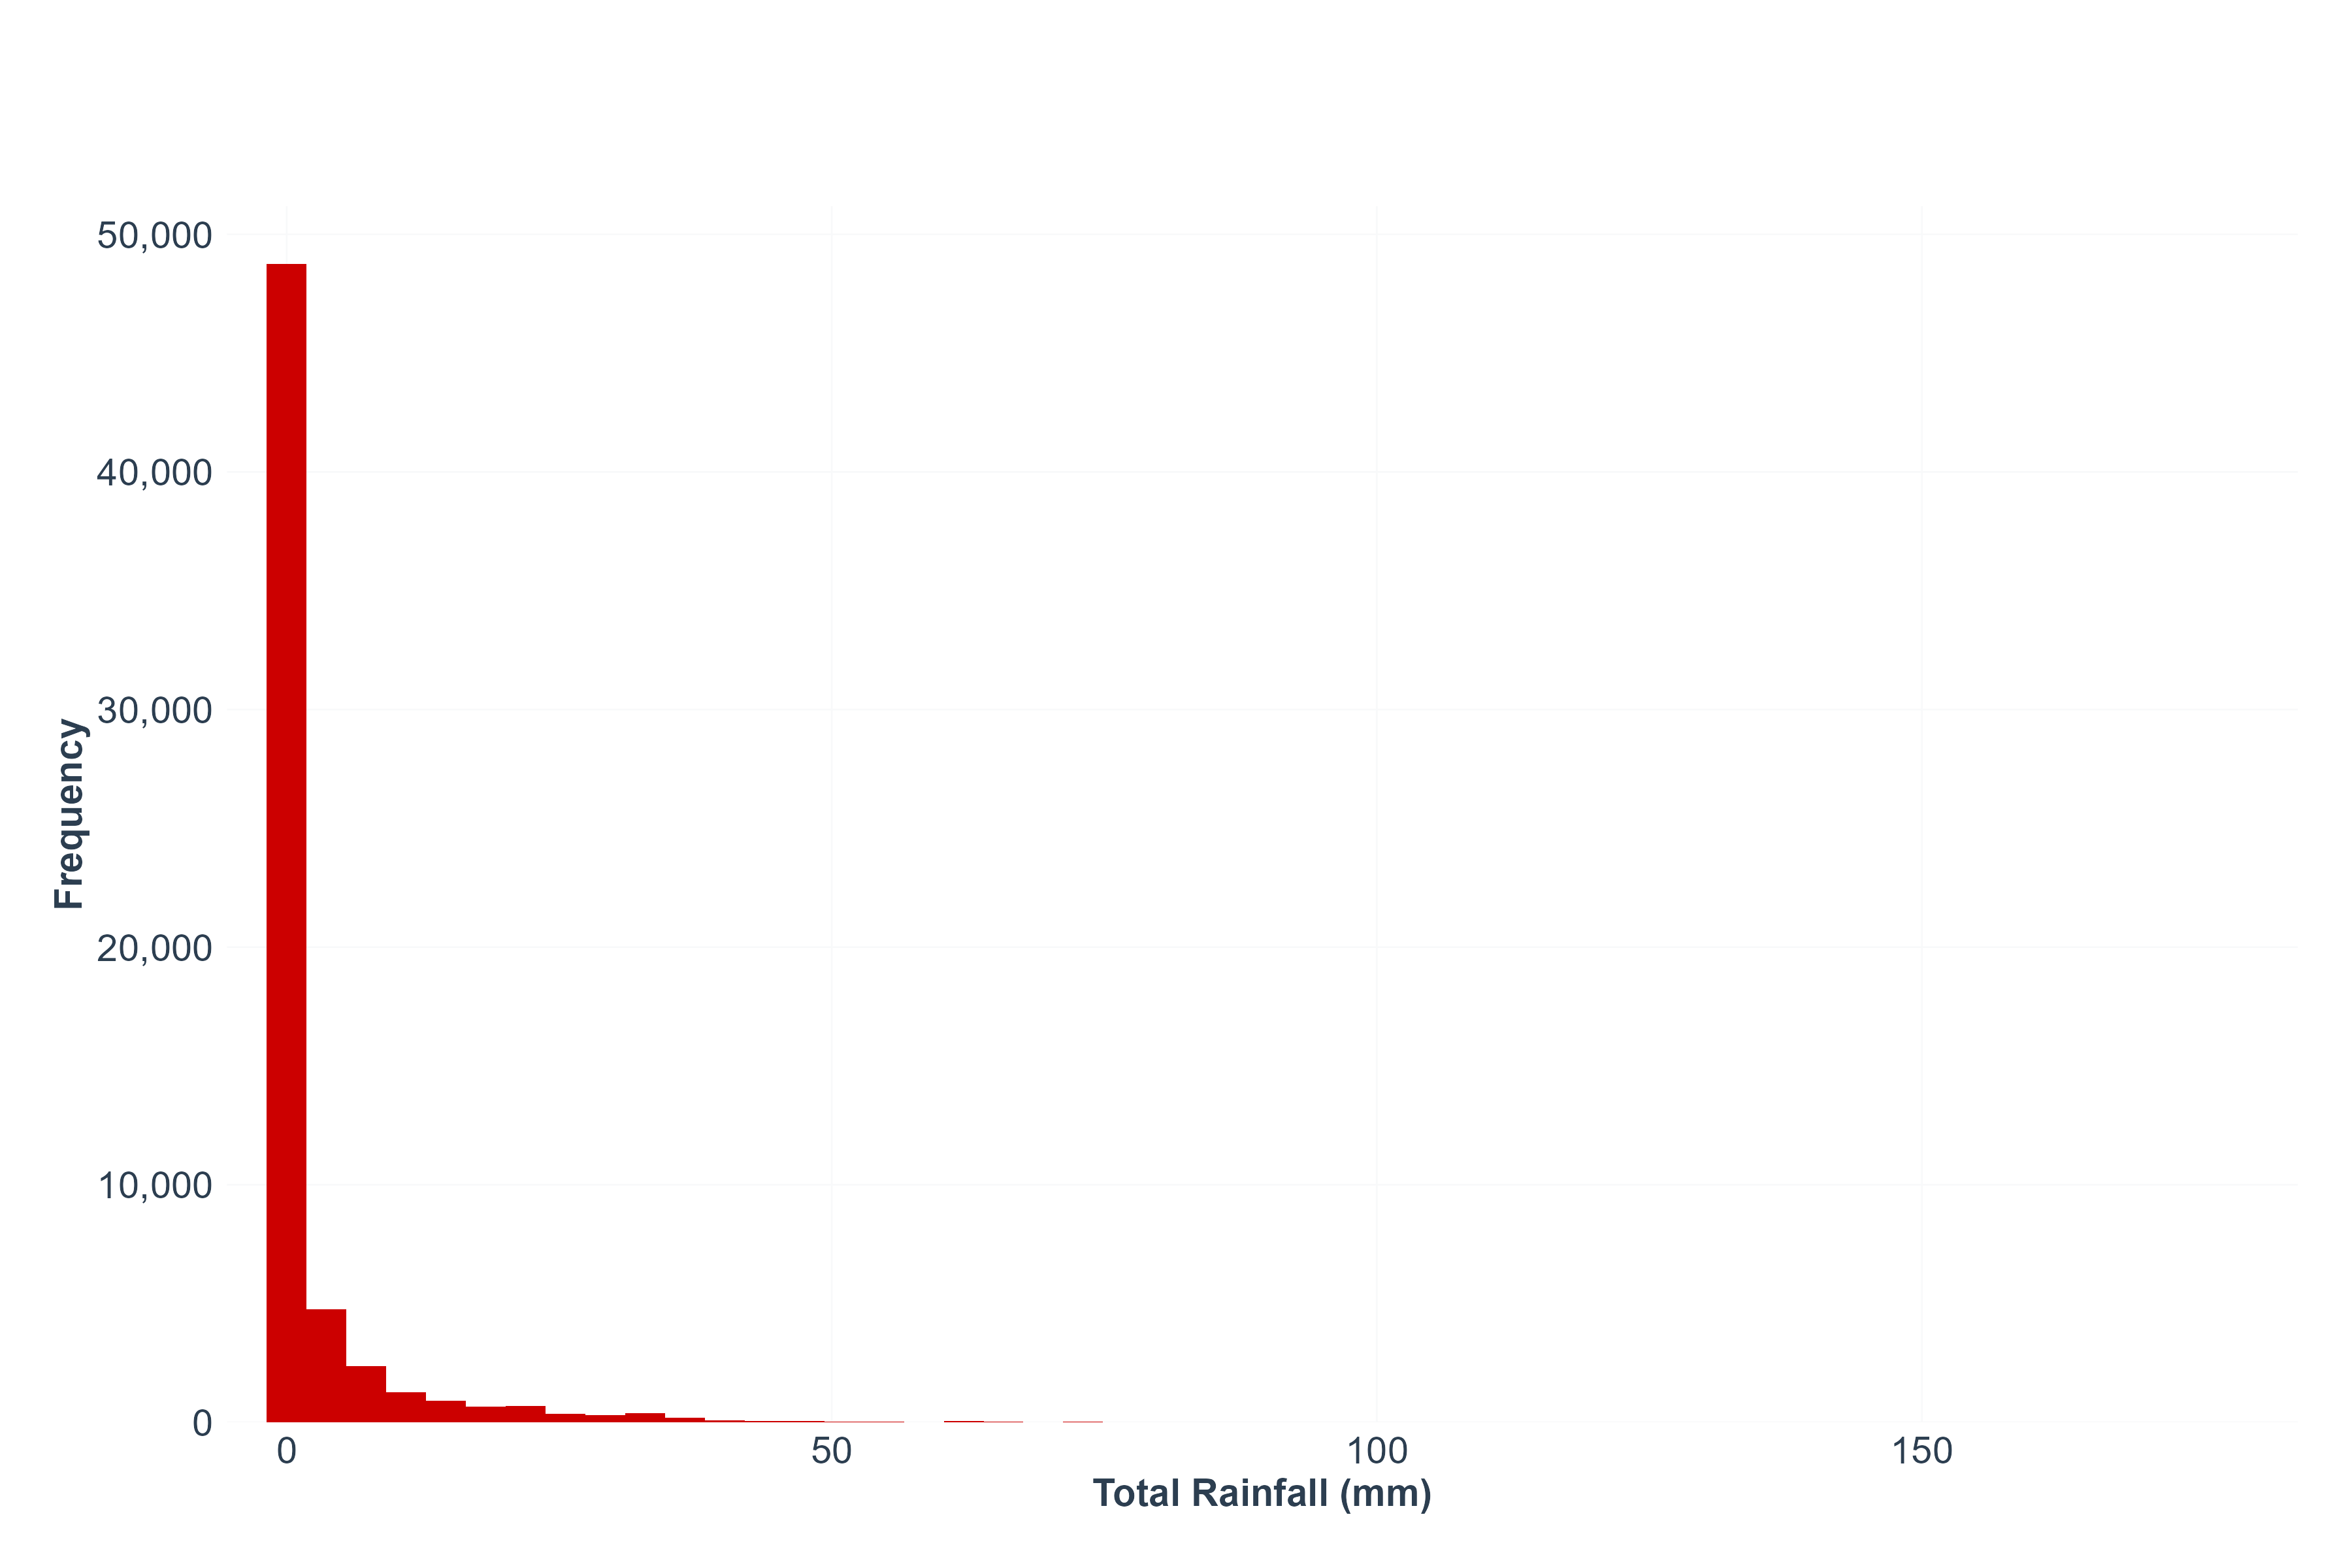
\includegraphics[width=0.8\textwidth]{../figures/rainfall_histogram.png}
    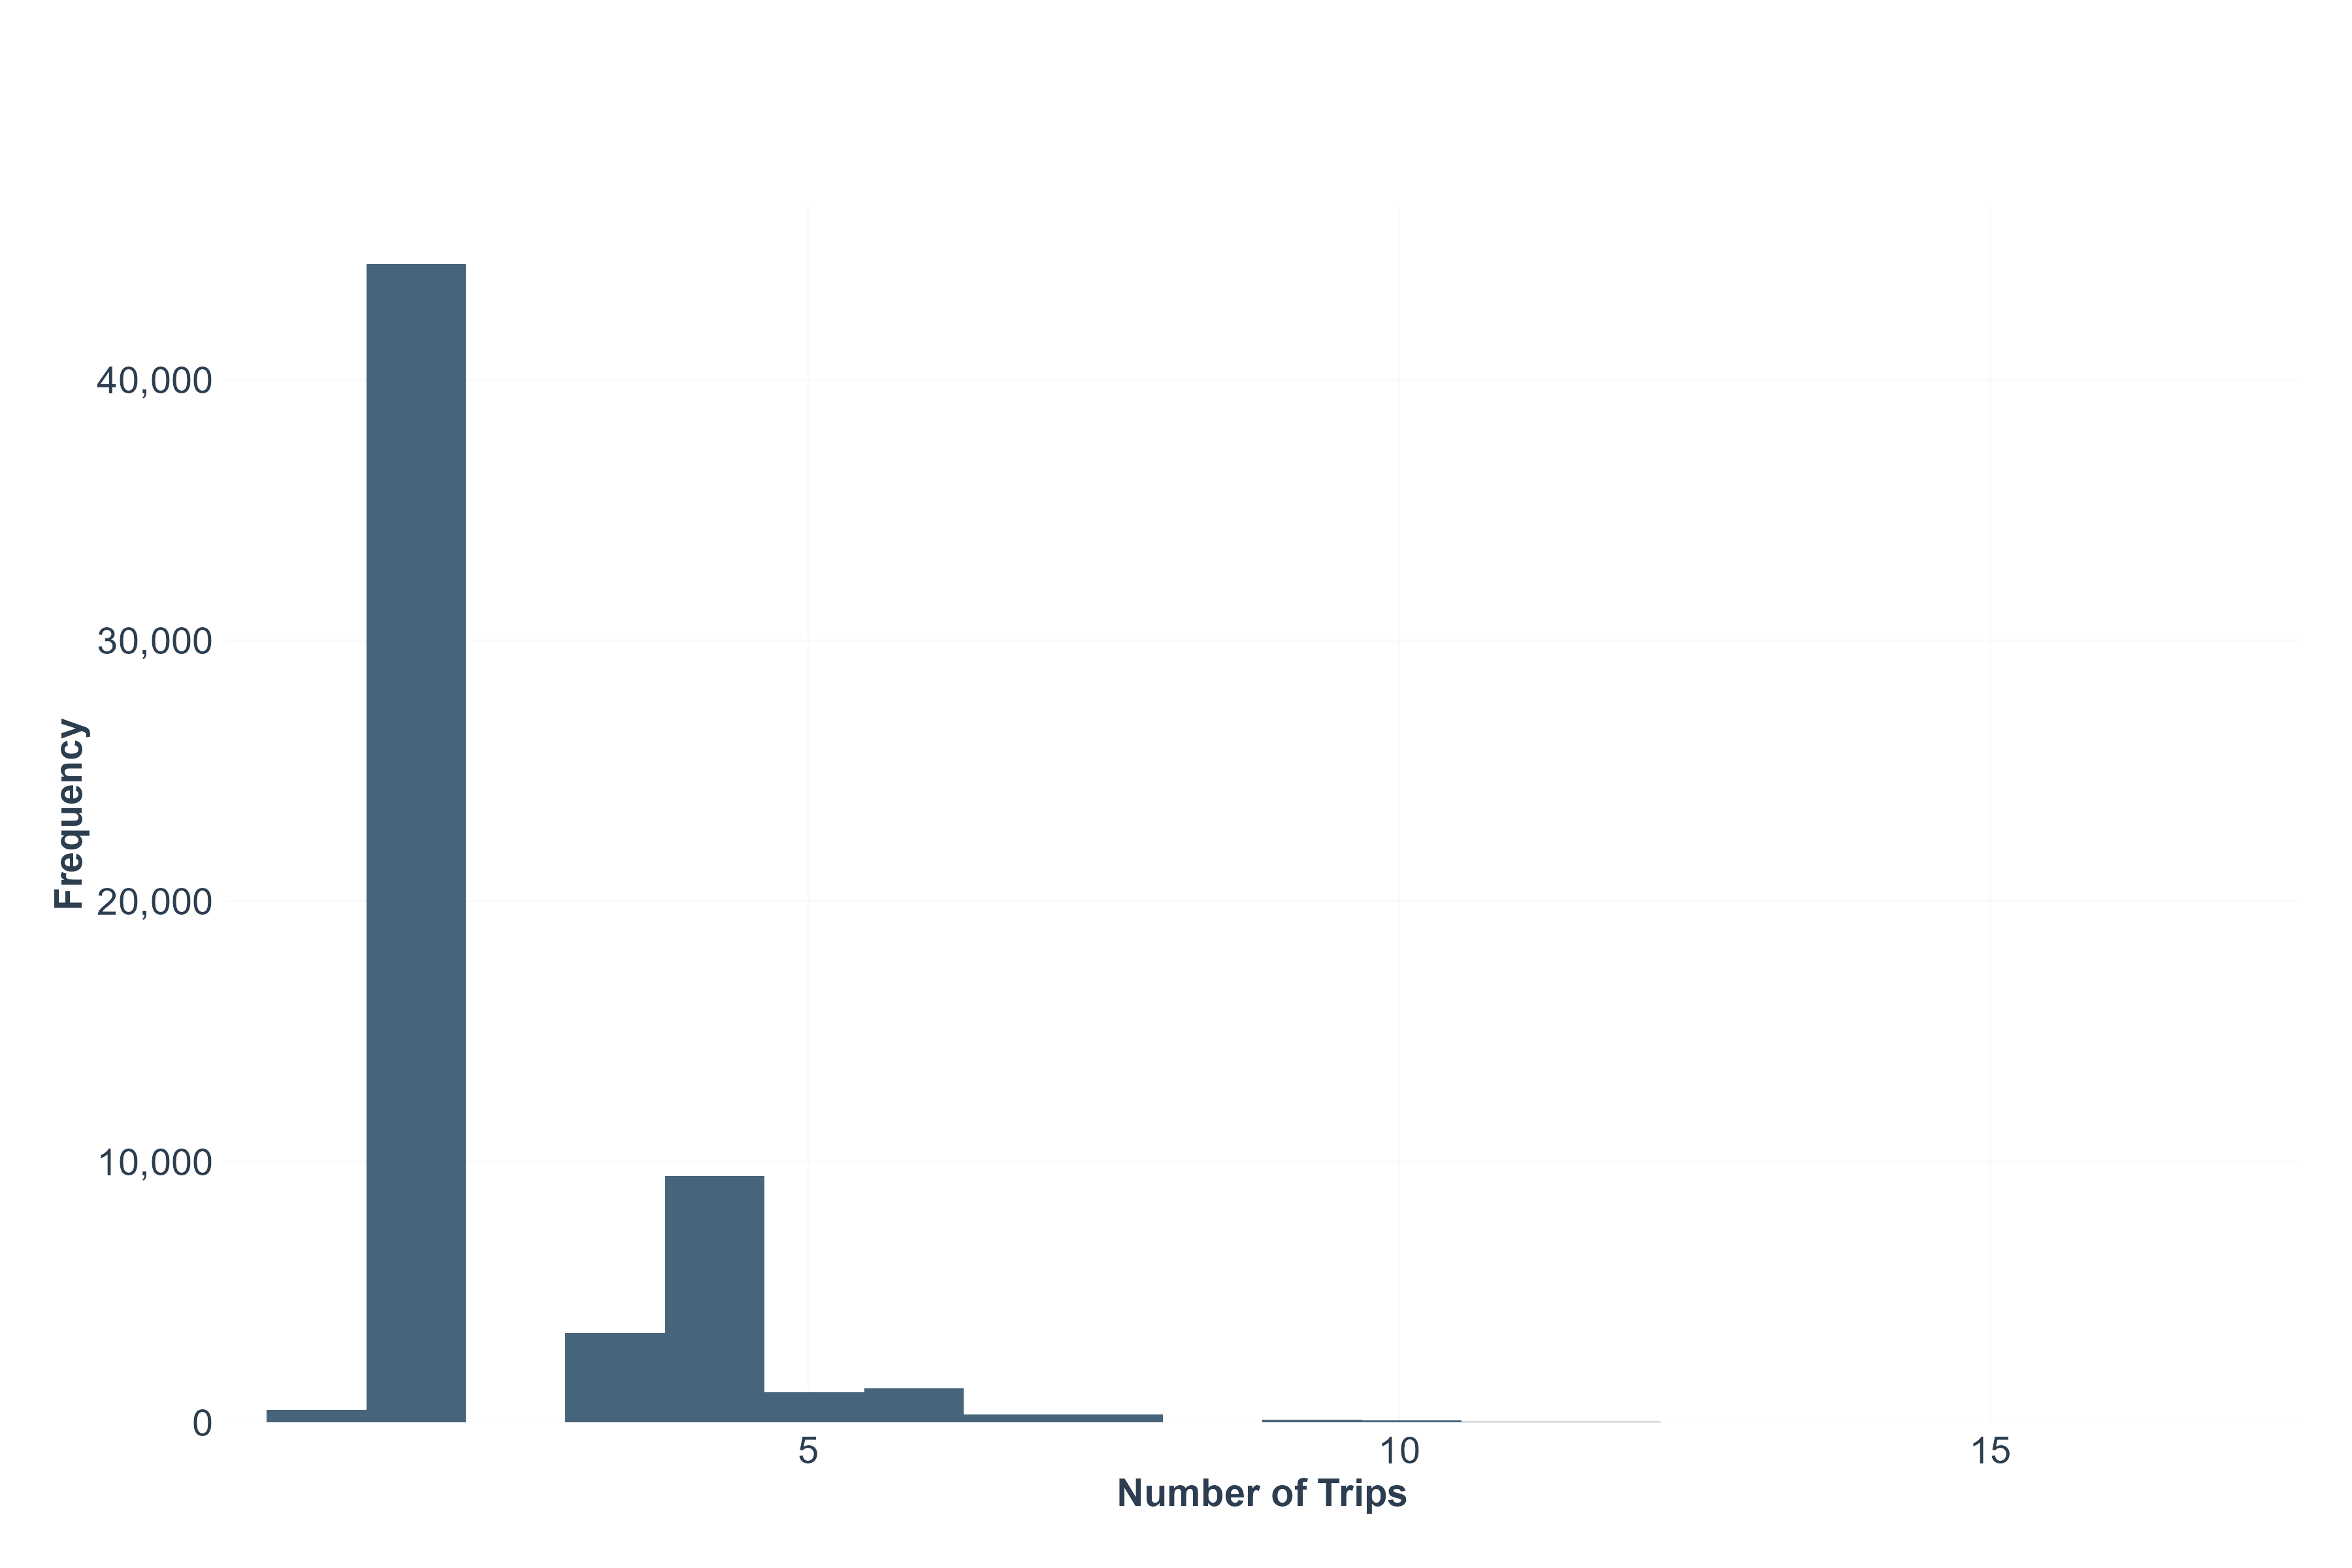
\includegraphics[width=0.8\textwidth]{../figures/trips_histogram.png}
    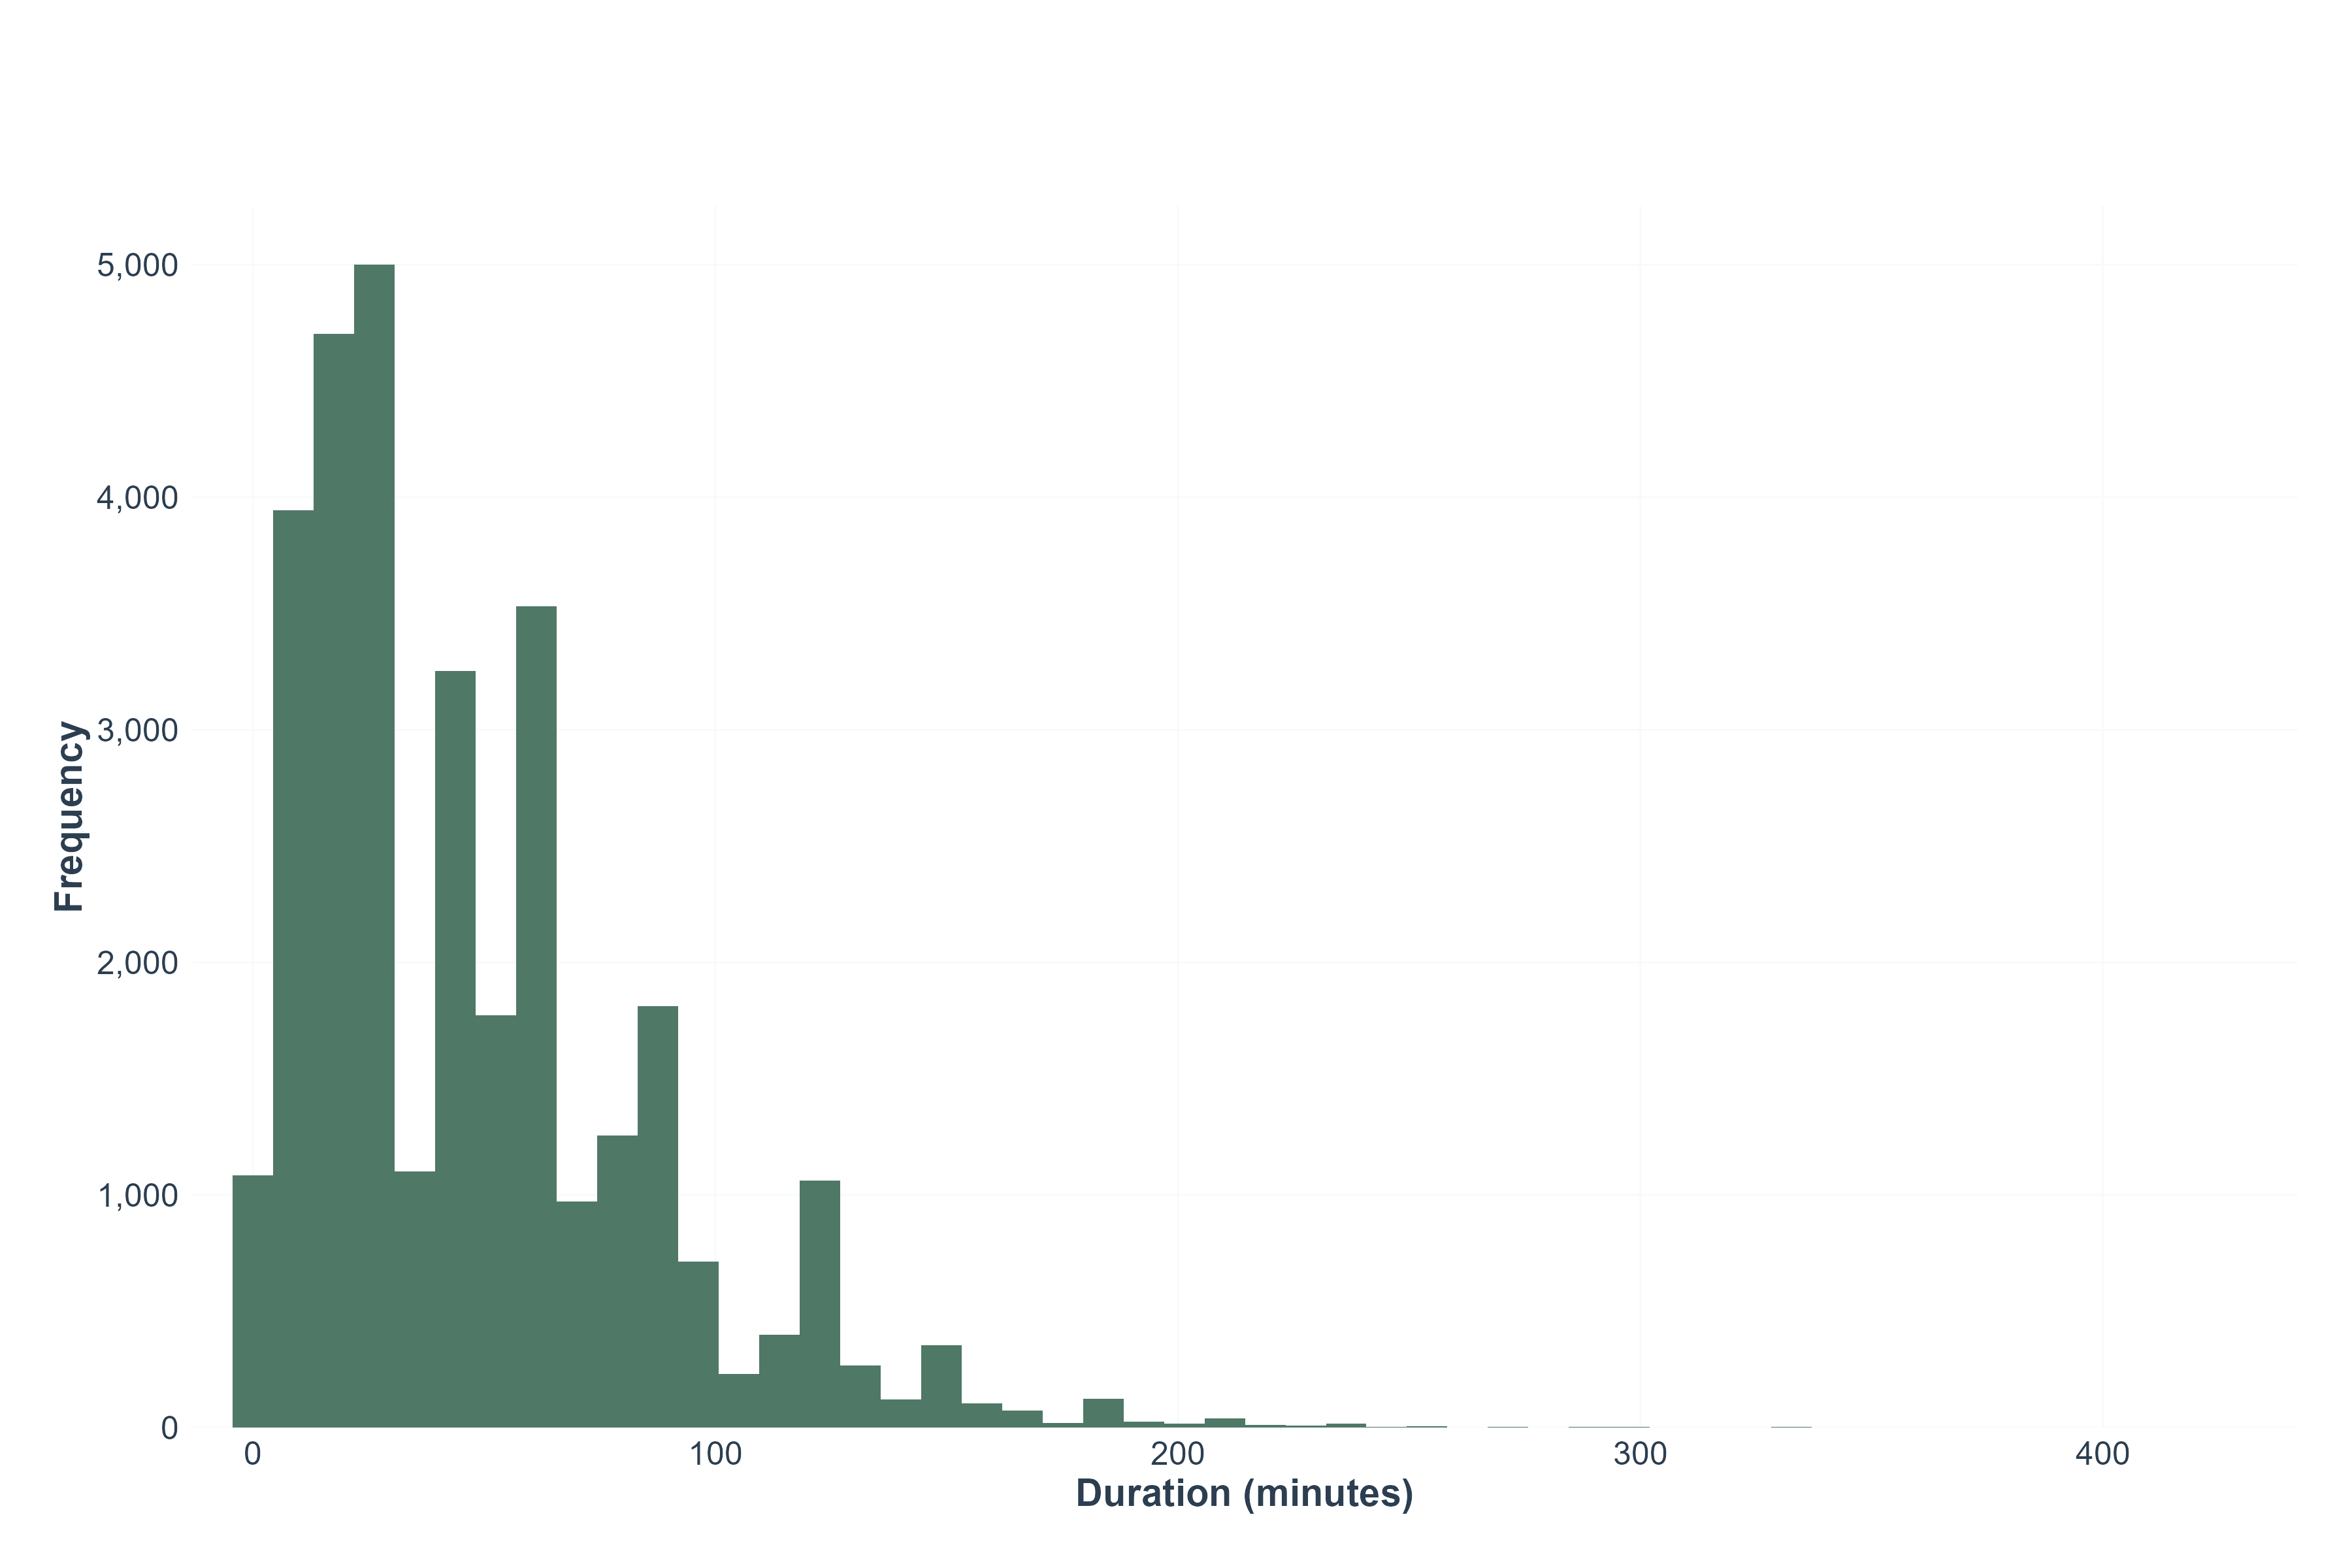
\includegraphics[width=0.8\textwidth]{../figures/duration_histogram.png}
    \caption{Histograms showing the distributions of rainfall (top), number of trips (middle), and commute durations (bottom) in the dataset.}
    \label{fig:hist}
\end{figure}

\begin{figure}[H]
    \centering
    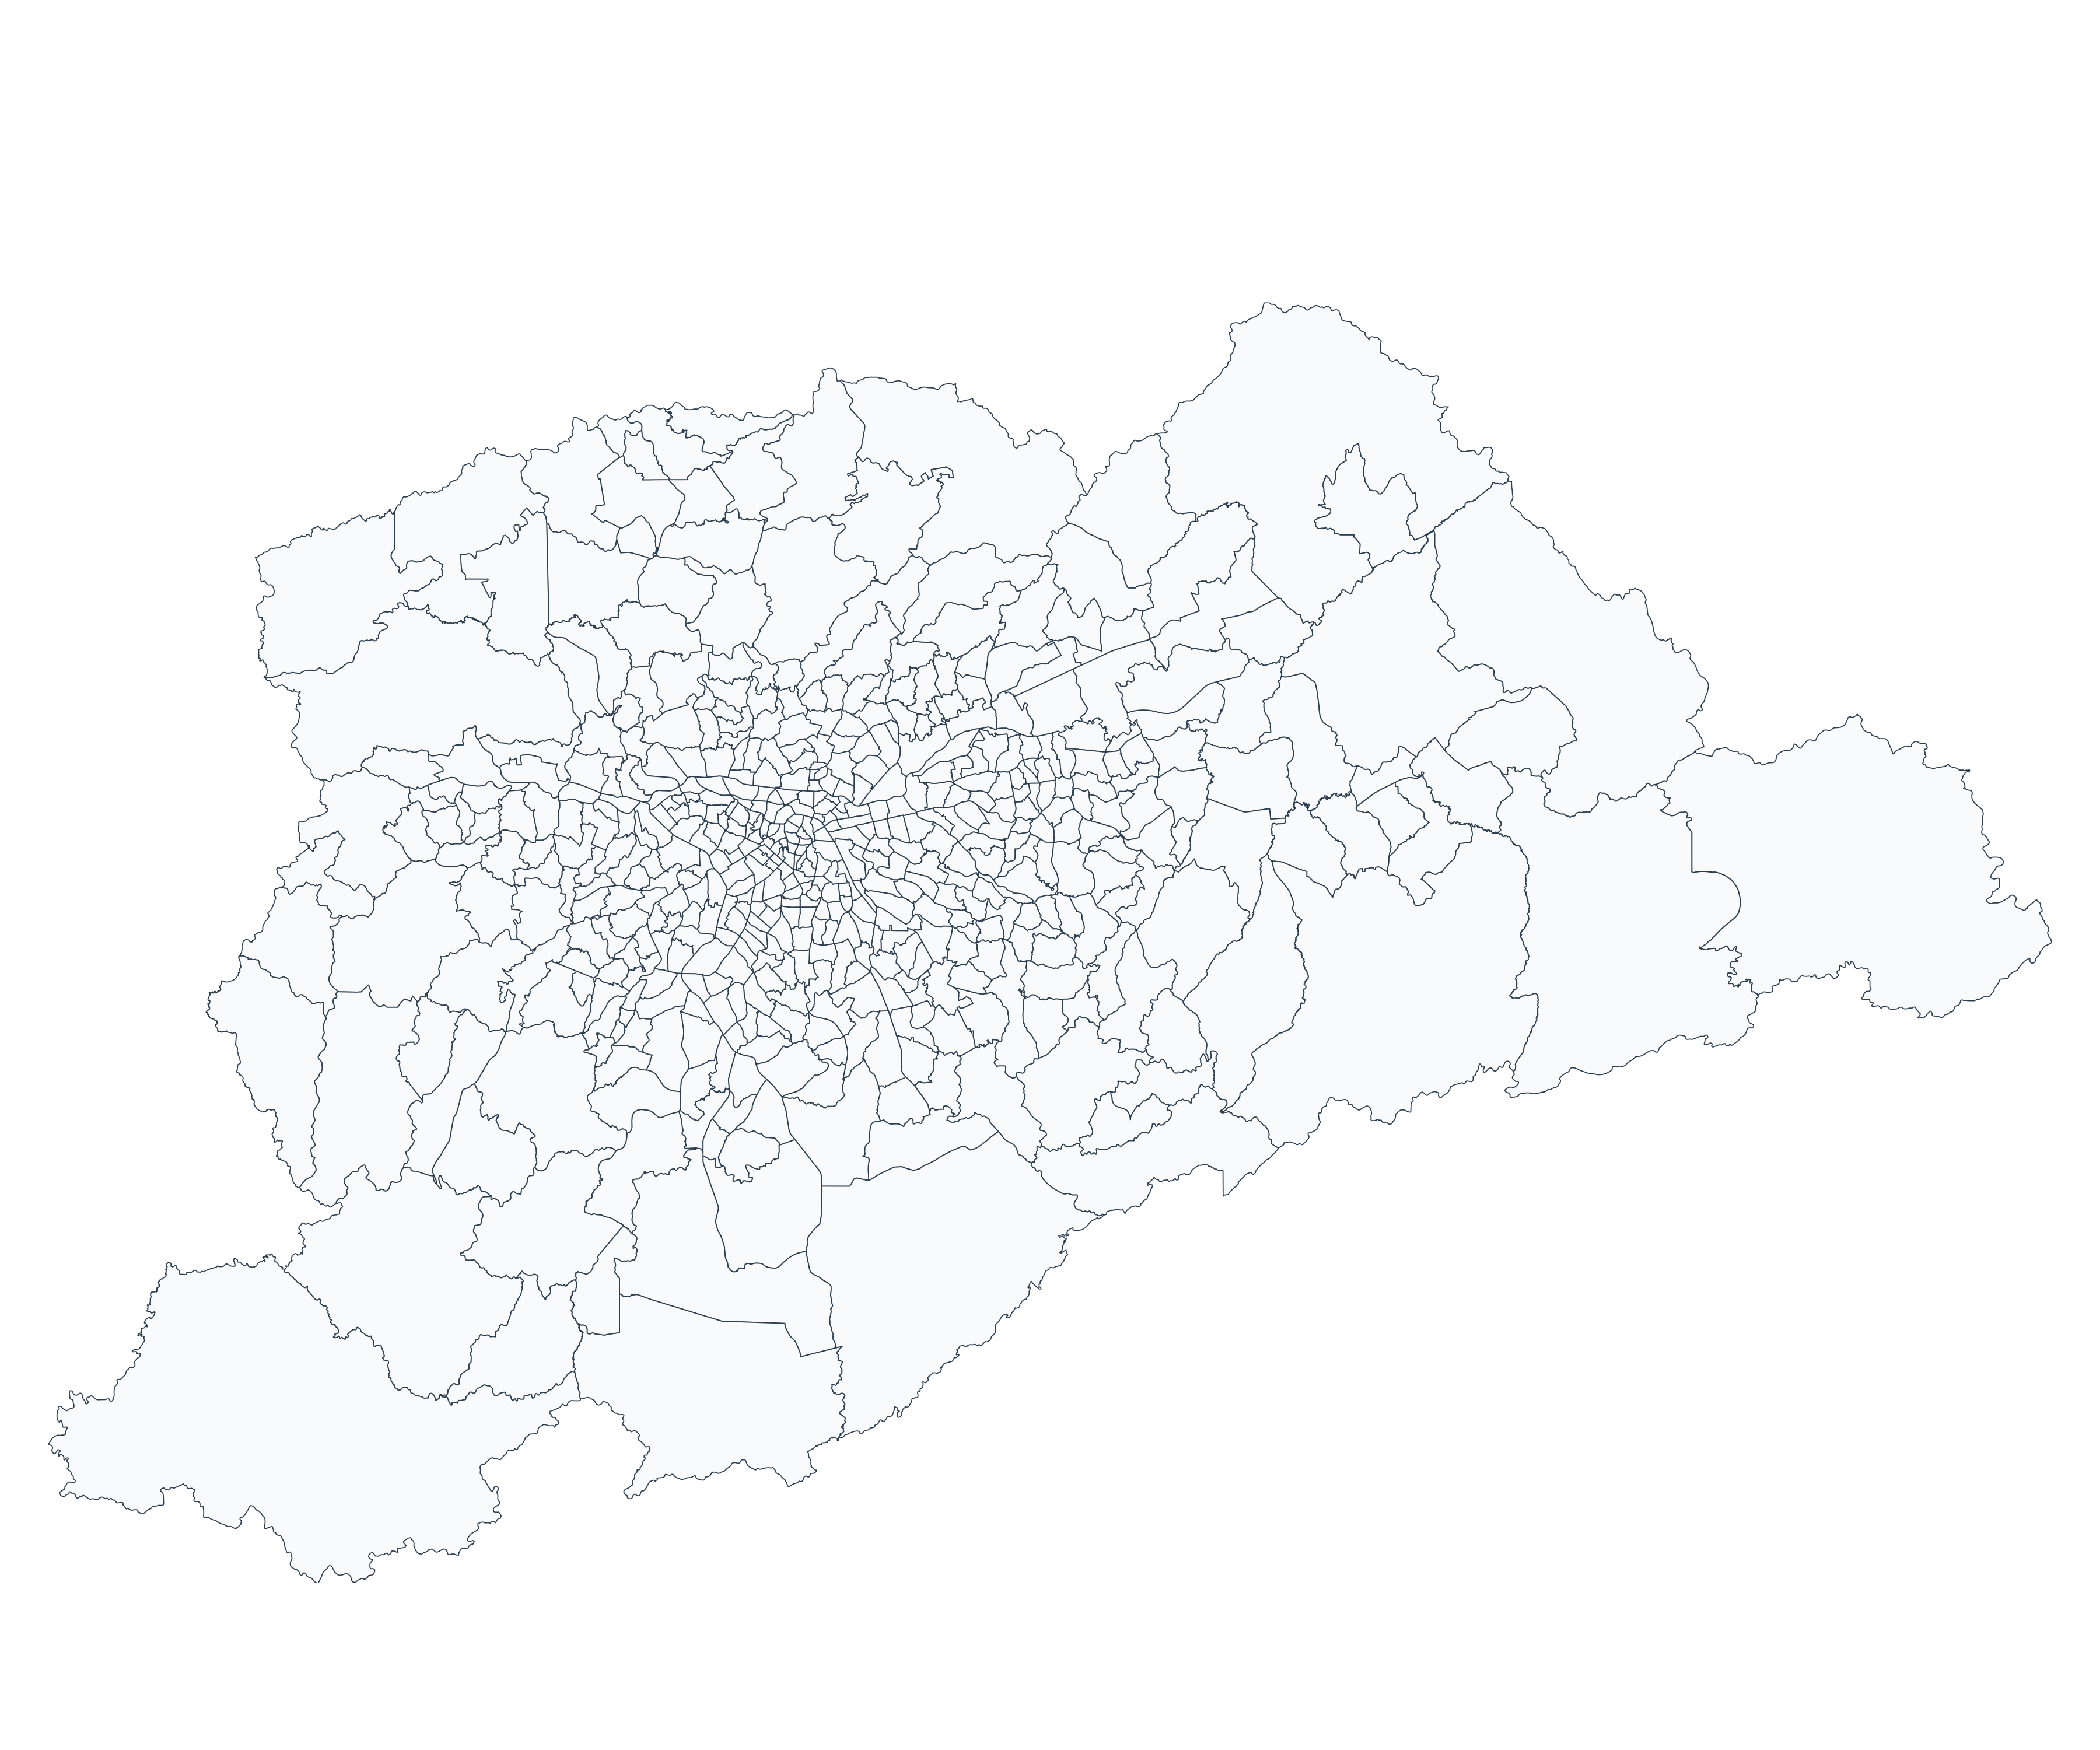
\includegraphics[width=0.8\textwidth]{../figures/rmsp_base.png}
    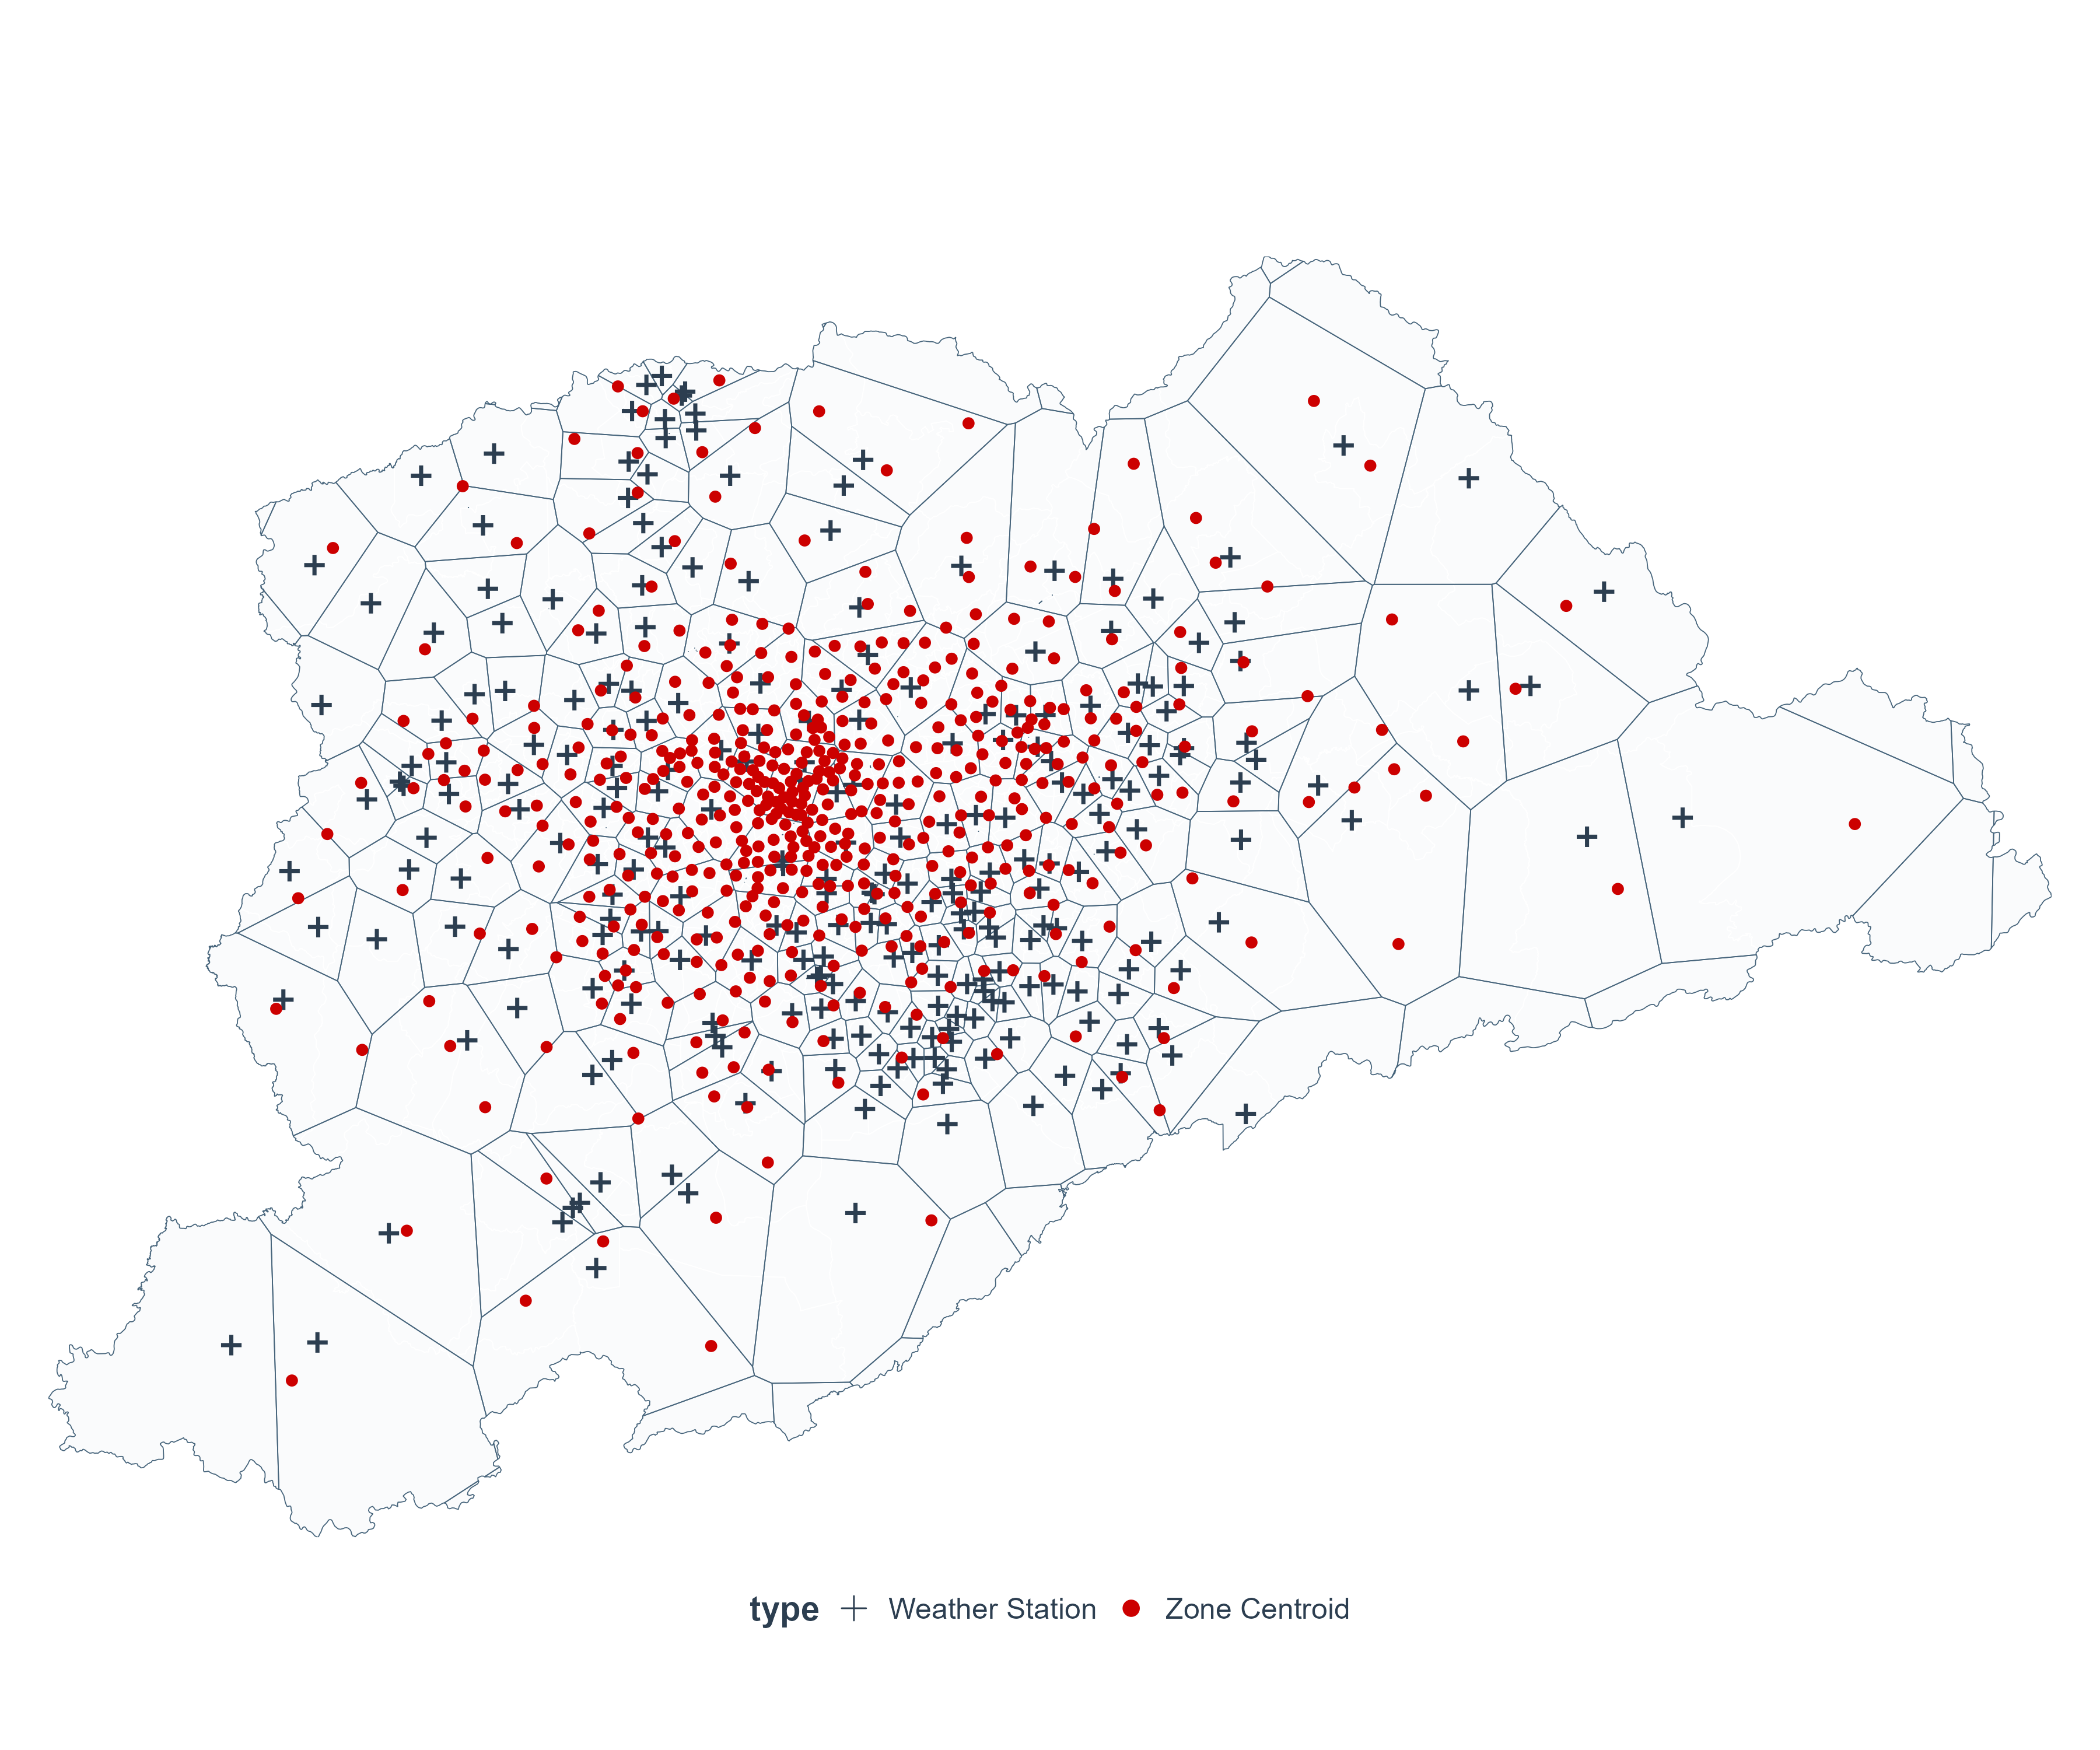
\includegraphics[width=0.8\textwidth]{../figures/rmsp_voronoi.png}
    \caption{Spatial representation of the RMSP region: (top) zone partitions, (bottom) Voronoi diagram illustrating spatial partitions based on centroid proximity to weather stations.}
    \label{fig:rmsp_voronoi}
\end{figure}

\label{tab:panel_a}
\begin{table}
\centering
\begin{talltblr}[         %% tabularray outer open
caption={Effect of Rainfall on Work Probability},
note{}={* p \num{< 0.1}, ** p \num{< 0.05}, *** p \num{< 0.01}},
note{ }={Sample consists of individuals regularly employed or do side gigs who worked on reference day. The dependent variable is a binary indicator equal to 1 if the individual worked on the reference day, 0 otherwise. Individual controls include age, gender dummy, education level, activity status, occupation, economic sector, and employment type. Zone fixed effects control for time-invariant spatial characteristics. Standard errors are heteroskedasticity-robust (HC1) and are shown in parentheses.},
]                     %% tabularray outer close
{                     %% tabularray inner open
colspec={Q[]Q[]Q[]Q[]Q[]Q[]},
column{2,3,4,5,6}={}{halign=c,},
column{1}={}{halign=l,},
hline{6}={1,2,3,4,5,6}{solid, black, 0.05em},
}                     %% tabularray inner close
\toprule
& Model 1 & Model 2 & Model 3 & Model 4 & Model 5 \\ \midrule %% TinyTableHeader
Rain Dummy (>0mm) & \num{-0.004} &  & \num{-0.004} & \num{-0.003} & \num{-0.001} \\
& (\num{0.003}) &  & (\num{0.004}) & (\num{0.004}) & (\num{0.004}) \\
Total Rainfall (mm) &  & \num{-0.000} & \num{0.000} & \num{-0.000} & \num{-0.000} \\
&  & (\num{0.000}) & (\num{0.000}) & (\num{0.000}) & (\num{0.000}) \\
Num.Obs. & \num{35488} & \num{35488} & \num{35488} & \num{35482} & \num{35482} \\
Individual Controls & No & No & No & Yes & Yes \\
Zone Fixed Effects & No & No & No & No & Yes \\
\bottomrule
\end{talltblr}

\end{table}

\label{tab:panel_b}
\begin{table}
\centering
\begin{talltblr}[         %% tabularray outer open
caption={Effect of Rainfall on Commute Duration},
note{}={* p \num{< 0.1}, ** p \num{< 0.05}, *** p \num{< 0.01}},
note{ }={Sample consists of individuals regularly employed or do side gigs who worked on reference day. The dependent variable is commute duration in minutes. Individual controls include age, gender dummy, education level, activity status, occupation, economic sector, and employment type. Zone fixed effects control for time-invariant spatial characteristics. Standard errors are heteroskedasticity-robust (HC1) and are shown in parentheses.},
]                     %% tabularray outer close
{                     %% tabularray inner open
colspec={Q[]Q[]Q[]Q[]Q[]Q[]},
column{2,3,4,5,6}={}{halign=c,},
column{1}={}{halign=l,},
hline{6}={1,2,3,4,5,6}{solid, black, 0.05em},
}                     %% tabularray inner close
\toprule
& Model 1 & Model 2 & Model 3 & Model 4 & Model 5 \\ \midrule %% TinyTableHeader
Rain Dummy (>0mm) & \num{-0.925}** &  & \num{-0.864}* & \num{-0.295} & \num{-0.144} \\
& (\num{0.436}) &  & (\num{0.488}) & (\num{0.473}) & (\num{0.483}) \\
Total Rainfall (mm) &  & \num{-0.035} & \num{-0.009} & \num{-0.023} & \num{0.019} \\
&  & (\num{0.031}) & (\num{0.034}) & (\num{0.033}) & (\num{0.034}) \\
Num.Obs. & \num{31715} & \num{31715} & \num{31715} & \num{31711} & \num{31711} \\
Individual Controls & No & No & No & Yes & Yes \\
Zone Fixed Effects & No & No & No & No & Yes \\
\bottomrule
\end{talltblr}

\end{table}
